%==============================================================================
%  Trajectories of point-based spatial analysis
%  Systematic review manuscript — LaTeX source
%
%  Build:  pdflatex main  ->  bibtex main  ->  pdflatex main  ->  pdflatex main
%==============================================================================
\documentclass[11pt,a4paper]{article}

\usepackage[T1]{fontenc}
\usepackage[utf8]{inputenc}
\usepackage{lmodern}
\usepackage[margin=2.5cm]{geometry}
\usepackage{graphicx}
\usepackage{booktabs}
\usepackage{longtable}
\usepackage{amsmath,amssymb}
\usepackage{natbib}
\usepackage{url}
\usepackage{hyperref}
\usepackage{setspace}
\usepackage{caption}
\usepackage{authblk}

\bibliographystyle{apalike}
\hypersetup{colorlinks=true, linkcolor=black, citecolor=black, urlcolor=blue}
\captionsetup{font=small, labelfont=bf}
\graphicspath{{../figures/}}
\onehalfspacing

\title{\textbf{Trajectories of point-based spatial analysis: a systematic
review of methods, application domains and case-study geographies,
1977--2026}}

\author[1]{Mohsen Roohani}
\affil[1]{\small Affiliation to be completed}

\date{}

\begin{document}
\maketitle

%------------------------------------------------------------------ HIGHLIGHTS
\section*{Highlights}
\begin{itemize}\itemsep2pt
  \item Systematic review of 223 studies applying point-based spatial
        analysis across nine application domains.
  \item Four convergent trajectories: description $\rightarrow$ inference,
        planar $\rightarrow$ constrained, statistics $\rightarrow$ learning,
        single $\rightarrow$ combined methods.
  \item Point process models overtook kernel density estimation as the modal
        analytical framework after 2015.
  \item Machine-learning components appear in 26\% of studies published since
        2020, but in none before 2006.
  \item Evidence is geographically concentrated: five countries supply 54\% of
        case studies; low-income countries supply 1.2\%.
\end{itemize}

%------------------------------------------------------------------- ABSTRACT
\section*{Abstract}
\noindent
\textbf{Background.} Point-based spatial analysis --- the family of methods
that treats the recorded locations of individual events as realisations of a
spatial point process --- underpins evidence in public health, ecology,
criminology, transport safety, seismology and archaeology. These literatures
have developed largely in parallel, and no synthesis has established whether
they are converging on a common methodological core.

\noindent
\textbf{Objectives.} To characterise how point-based spatial analysis has
developed over five decades, and to map its methods, application domains and
case-study geographies.

\noindent
\textbf{Methods.} We conducted a systematic review following PRISMA 2020.
Fourteen structured queries were issued to a federated bibliographic index
spanning Semantic Scholar, PubMed, Scopus and arXiv on 28 July 2026, returning
278 records. After duplicate removal and eligibility assessment, 223 studies
were included. Each was coded for method family, application domain,
case-study country and temporal dimension. Synthesis was narrative and
quantitative, with trajectories analysed by publication period.

\noindent
\textbf{Results.} Included studies span 1977--2026; 58\% were published from
2020 onward. Parametric point process models were the most widely used family
(73 studies, 33\%), overtaking kernel density estimation (66, 30\%) as the
modal analytical framework after 2015. Three-quarters of studies (75\%)
combined two or more method families, and network-constrained formulations
appeared in 13\%. Machine-learning components were absent before 2006 but
appeared in 26\% of studies published since 2020. Public health (46 studies)
and ecology (45) dominated, but methodological exchange between domains was
substantial. Case studies covered 49 countries, with pronounced concentration:
the United States, China, the United Kingdom, Japan and Brazil together
supplied 54\% of country-attributable studies, high-income countries 56\%, and
low-income countries 1.2\%.

\noindent
\textbf{Conclusions.} Point-based spatial analysis is converging on a shared
inferential core built on point process models, but the convergence is uneven
and its empirical base is geographically narrow. Priorities are transparent
reporting of bandwidth, edge-correction and null-model choices; explicit
treatment of geocoding uncertainty; and deliberate investment in
under-represented geographies.

\vspace{6pt}
\noindent\textbf{Keywords:} spatial point process; point pattern analysis;
kernel density estimation; scan statistic; linear network; spatio-temporal
modelling; systematic review; PRISMA

\newpage
%--------------------------------------------------------------- INTRODUCTION
\section{Introduction}

A great deal of what is known about where things happen rests on datasets of
individual, georeferenced events: the residence of a person at diagnosis, the
stem of a tree in a mapped plot, the location of a burglary, a crash, an
earthquake epicentre, an ignition, a potsherd. The statistical machinery for
analysing such data --- spatial point pattern analysis --- was formalised in
the 1970s \citep{ripley1977} and consolidated through a sequence of
monographs that remain the field's reference texts
\citep{diggle2013a,illian2008,baddeley2015,wiegand2013}. Its central idea is
simple and unusually general: treat the observed configuration of points as
one realisation of a stochastic process, and ask what that realisation implies
about the process that generated it.

That generality is the source of both the field's reach and its fragmentation.
The same second-order summary function that a plant ecologist uses to detect
conspecific aggregation \citep{haase1995,perry2006,law2009} is used by a
criminologist to test whether burglaries cluster along a street network
\citep{khalid2017}, and by a seismologist to characterise aftershock
triggering \citep{ogata2006}. Yet these communities cite different
methodological literatures, adopt different software, and report different
diagnostics. Domain-specific reviews exist --- for point pattern analysis in
ecology \citep{velazquez2016,bensaid2021}, for scan statistics in
low- and middle-income country health research \citep{aboushady2025}, for
point patterns on linear networks \citep{baddeley2020}, for self-exciting
processes \citep{reinhart2017,bernabeu2024} --- but each looks along a single
axis. Whether the field as a whole is converging on shared methodology, or
diverging into mutually unintelligible dialects, has not been established
systematically.

This matters for three reasons. First, methodological choices that are
well-understood in one domain are repeatedly rediscovered in another: the
sensitivity of kernel density estimates to bandwidth, established in crime
mapping two decades ago \citep{chainey2008,chainey2014,hart2014}, resurfaces as
a novel concern in violence-prevention research \citep{zewdie2025}. Second,
methods that resolve known pathologies --- network-constrained estimation for
events confined to roads \citep{okabe2009,baddeley2020}, inhomogeneous
summary functions for environmentally heterogeneous landscapes
\citep{law2009,wiegand2007} --- diffuse slowly and unevenly. Third, if the
empirical base is drawn from a narrow set of countries, then what the field
believes about spatial processes is conditioned on where it happens to have
looked.

We therefore ask four questions. \textbf{(Q1)} Which method families
constitute point-based spatial analysis, and how has their relative use
changed over time? \textbf{(Q2)} Do method families remain siloed within
application domains, or is there systematic cross-domain exchange?
\textbf{(Q3)} Is there evidence of methodological maturation --- greater
temporal explicitness, greater methodological breadth, uptake of statistical
learning? \textbf{(Q4)} What is the geography of the evidence base, and how is
it distributed across world regions and national income groups?

Our contribution is a cross-domain, quantitative synthesis of 223 studies
spanning 1977--2026, with a reproducible coding framework, a complete
extraction dataset, and analysis code released alongside the manuscript.

%-------------------------------------------------------------------- METHODS
\section{Methods}

\subsection{Protocol and reporting}
The review was conducted and is reported in accordance with the PRISMA 2020
statement. The protocol, eligibility criteria and coding frame were specified
before synthesis and are distributed with the review dataset
(\texttt{protocol/}). The review was not prospectively registered; this is
noted as a limitation in Section~\ref{sec:limits}.

\subsection{Eligibility criteria}
Eligibility was defined on a Population--Concept--Context frame
(Table~\ref{tab:elig}). We included studies that analysed georeferenced
\emph{event locations} using at least one point-based spatial statistic or
point process model, in any application field, geography or period. We
excluded: analyses conducted exclusively on areal or lattice aggregates,
raster surfaces, or extended line/polygon objects; purely temporal point
process contributions with no spatial component; accessibility, travel-time
and site-suitability models applying no point pattern statistic; books,
monographs, theses, book reviews, correction notices and conference abstracts
without full text; and records whose indexed metadata were absent or
corrupted.

The distinction between point-based and areal analysis was applied strictly
and is the single most consequential judgement in the review. A study that
computed Getis--Ord $G_i^*$ on municipality-level ignition counts was
excluded; a study that computed the same statistic on network segments
carrying individual crash locations was included. This boundary is recorded
per record in the extraction dataset so that readers may re-draw it.

\subsection{Information sources and search strategy}
Searches were executed on 28 July 2026 against a federated bibliographic index
covering Semantic Scholar, PubMed, Scopus and arXiv. Fourteen structured
queries (Table~\ref{tab:search}) were constructed on a method $\times$ domain
matrix, so that each principal method family and each principal application
domain was addressed by at least one query. Queries were natural-language
rather than Boolean, reflecting the retrieval interface; the exact strings are
reported verbatim to support replication.

We were unable to obtain native Scopus or Web of Science exports, and no
citation-chaining or hand-searching of reference lists was performed. The
implications are addressed in Section~\ref{sec:limits}.

\subsection{Selection process}
Records were de-duplicated on normalised titles and on manual identification
of preprint/journal pairs and correction notices. Titles and abstracts were
then screened against the eligibility criteria, and an inclusion decision plus
a free-text exclusion reason recorded for every record. The complete decision
log, including all excluded records with reasons, is provided as
Supplementary Table~S2.

\subsection{Data extraction and coding framework}
For each included study we extracted: authorship, year, source title,
publication type, citation count, primary method family, all method families
applied, application domain, case-study country, and whether the analysis had
an explicit temporal dimension.

Method families (Table~\ref{tab:methods}) were coded into eleven categories
spanning kernel density estimation; second-order distance statistics
(Ripley's $K$, $L$, the pair correlation function $g$, and the $F$, $G$ and
$J$ functions); nearest-neighbour indices; scan statistics; local indicators
of spatial association applied to points; parametric point process models;
spatio-temporal and self-exciting processes; network-constrained analysis;
co-location and marked pattern methods; machine-learning point models; and
other approaches. A study's \emph{primary} family is its dominant analytical
approach; \emph{all} families record every approach applied, so studies
contribute to more than one family where appropriate.

Case-study countries were assigned only where a specific national study area
was identifiable from the record. Methodological contributions, simulation
studies and multi-country analyses were coded as not attributable, multiple,
or not specified, and excluded from country-level analyses. Countries were
grouped into world regions and into World Bank-style income groups for the
equity analysis.

\subsection{Synthesis}
Synthesis was narrative, supported by descriptive quantitative analysis.
Temporal trajectories were computed as annual counts smoothed with a
three-year centred moving average, and as compositional shares restricted to
years with an adequate publication base. Maturation indicators were compared
across four periods ($\leq$2005, 2006--2012, 2013--2019, 2020--2026). Method
co-occurrence was analysed as a weighted graph over the \emph{all families}
coding. Because the review synthesises methodological practice rather than
treatment effects, no meta-analysis of effect sizes and no risk-of-bias
assessment was appropriate; we instead report structured descriptors of
methodological completeness.

All analyses were performed in Python 3.11 (\texttt{pandas}, \texttt{numpy},
\texttt{networkx}, \texttt{matplotlib}). Code and data are available as
described under Data availability.

%-------------------------------------------------------------------- RESULTS
\section{Results}

\subsection{Study selection}
The 14 queries returned 278 records. Four were duplicates, leaving 274 for
screening. Fifty-one records were excluded, most commonly because no
point-based statistic was applied to event locations ($n=30$), because the
publication type was ineligible ($n=18$), or because the bibliographic record
was insufficient or corrupted ($n=3$). This left \textbf{223 included
studies} (Figure~\ref{fig:prisma}).

\begin{figure}[htbp]
\centering
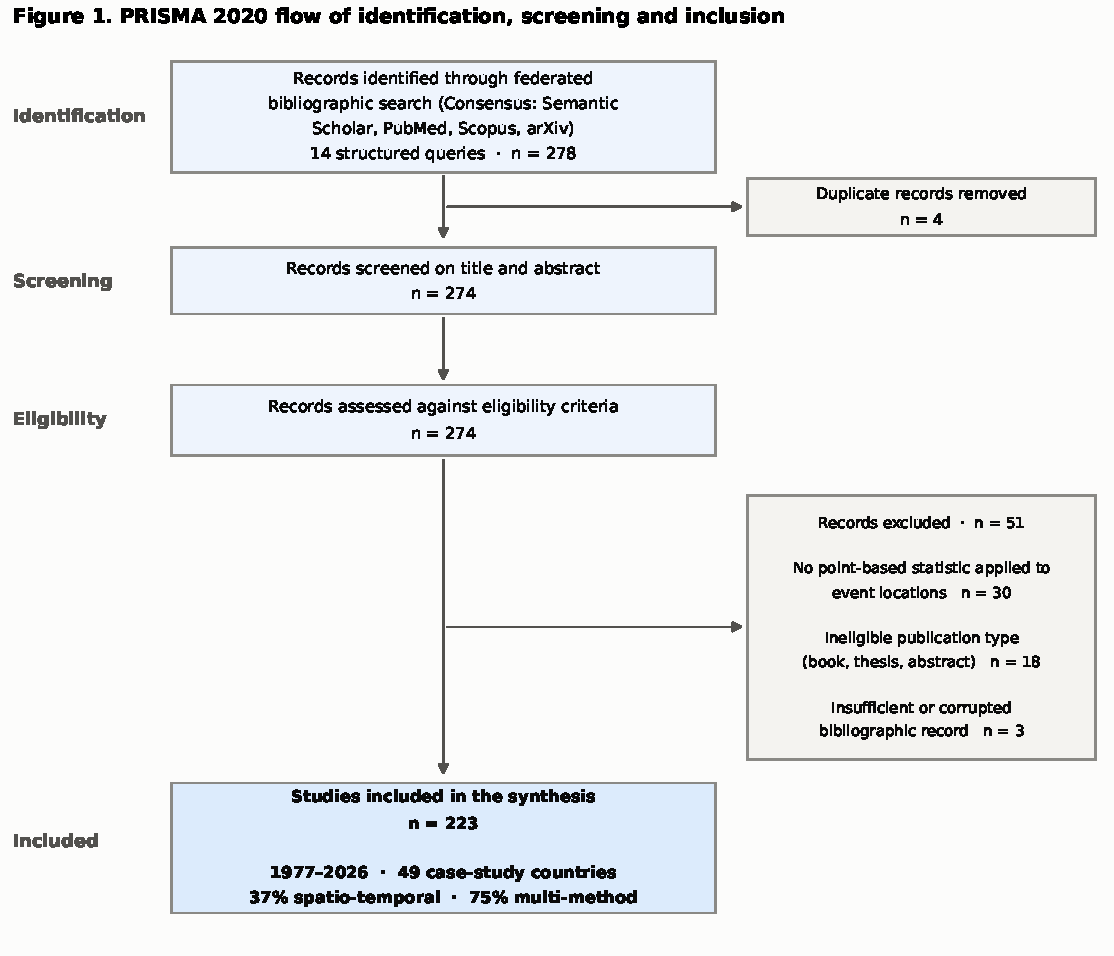
\includegraphics[width=0.78\linewidth]{fig01_prisma_flow.pdf}
\caption{PRISMA 2020 flow of identification, screening and inclusion.}
\label{fig:prisma}
\end{figure}

\subsection{Characteristics of the evidence base}
Included studies span 1977 to 2026, with a median publication year of 2021;
129 studies (57.8\%) appeared from 2020 onward (Table~\ref{tab:characteristics}).
Journal articles predominate, with conference papers and preprints
concentrated in the machine-learning literature. The median citation count is
18 (IQR 3--71), reflecting a mixture of recent applications and a small number
of heavily cited methodological anchors.

Two structural features stand out. First, 168 studies (75.3\%) applied two or
more method families, indicating that point-based analysis is typically
practised as a toolkit rather than as a single test. Second, only 83 studies
(37.2\%) modelled an explicit temporal dimension, so the majority of the field
remains purely spatial despite the wide availability of time-stamped event
data.

\subsection{Q1 --- Method families and their changing composition}
Parametric point process models are the most widely applied family (73
studies, 32.7\% of the corpus), followed by kernel density estimation (66,
29.6\%), spatio-temporal and self-exciting processes (57, 25.6\%),
second-order distance statistics (53, 23.8\%) and machine-learning point
models (51, 22.9\%) (Table~\ref{tab:methods}).

The temporal trajectory (Figure~\ref{fig:traj}) shows three phases. Before
about 2002 the literature is thin and dominated by second-order distance
statistics developed in plant ecology \citep{haase1995,perry2006}. From the
mid-2000s the field expands rapidly, initially through kernel density
estimation and scan statistics, which were carried into practice by
accessible software and a strong applied demand in crime mapping
\citep{chainey2008,nakaya2010} and disease surveillance
\citep{takahashi2008,coleman2009}. From roughly 2015 the composition shifts
again: point process models and, subsequently, machine-learning formulations
take an increasing share, while the relative weight of purely descriptive
density mapping declines.

\begin{figure}[htbp]
\centering
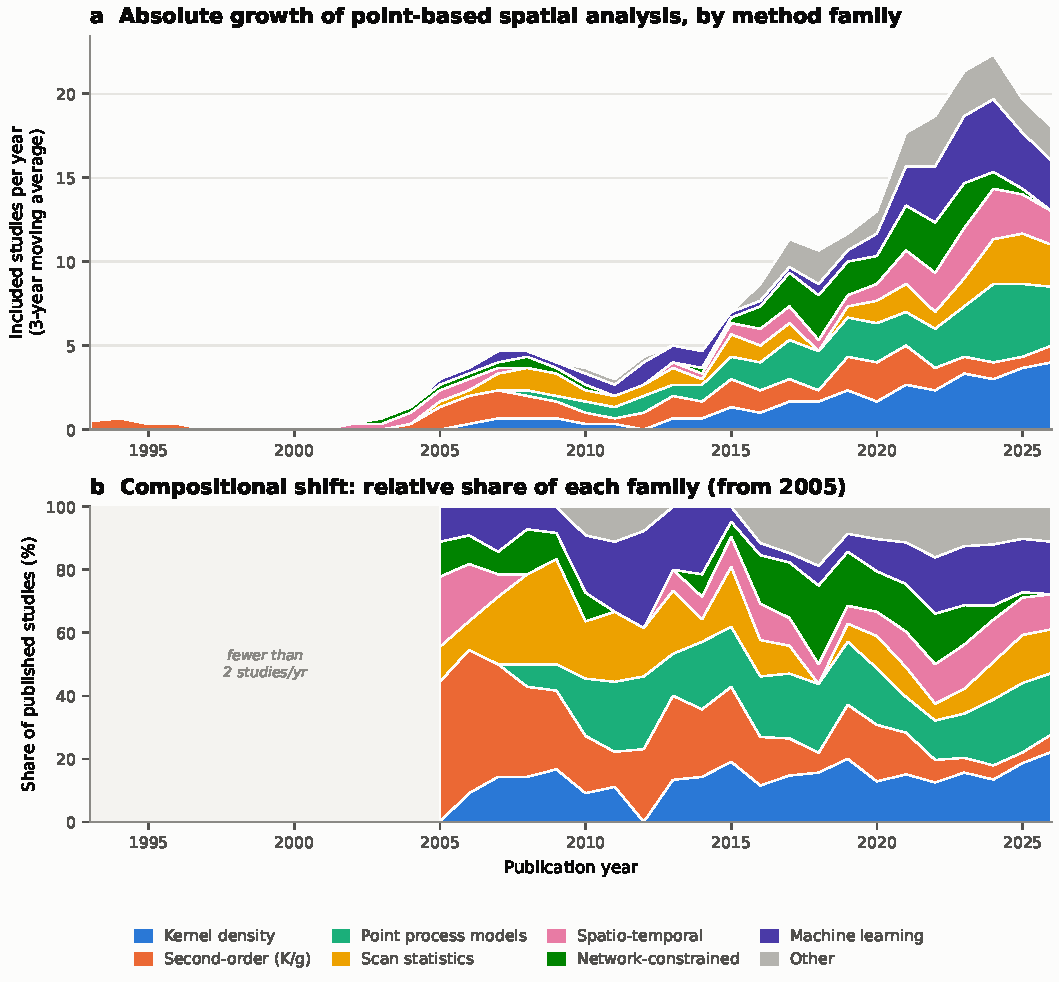
\includegraphics[width=\linewidth]{fig02_method_trajectory.pdf}
\caption{Growth and compositional change of point-based spatial analysis.
(a) Annual number of included studies by primary method family, three-year
centred moving average. (b) Relative share of each family, restricted to years
with at least two studies per year.}
\label{fig:traj}
\end{figure}

The substantive reading is a movement \emph{from description to inference}.
Kernel density estimation answers ``where is the intensity high?''; a fitted
log-Gaussian Cox process answers ``what covariates explain the intensity,
with what uncertainty, and does residual clustering remain?''
\citep{diggle2013b,li2012b,johnson2019,konstantinoudis2018a}. The
displacement is partial rather than total: kernel estimation persists because
it remains the natural exploratory first step and the natural communication
device, and it is increasingly used \emph{inside} inferential workflows --- as
an intensity estimate for an inhomogeneous null model, or as a covariate
surface --- rather than as a terminal result.

\subsection{Q2 --- Cross-domain exchange}
Method use is strongly but not exclusively structured by domain
(Figure~\ref{fig:heat}; Table~\ref{tab:crosstab}). Scan statistics are
overwhelmingly a public-health technology (21 of 25 studies with scan
statistics as the primary family). Second-order distance statistics are
concentrated in ecology (22 of 31). Network-constrained methods are
concentrated in road safety (12 of 23) and urban geography (6 of 23).
Spatio-temporal processes are concentrated in seismology (14 of 23).

\begin{figure}[htbp]
\centering
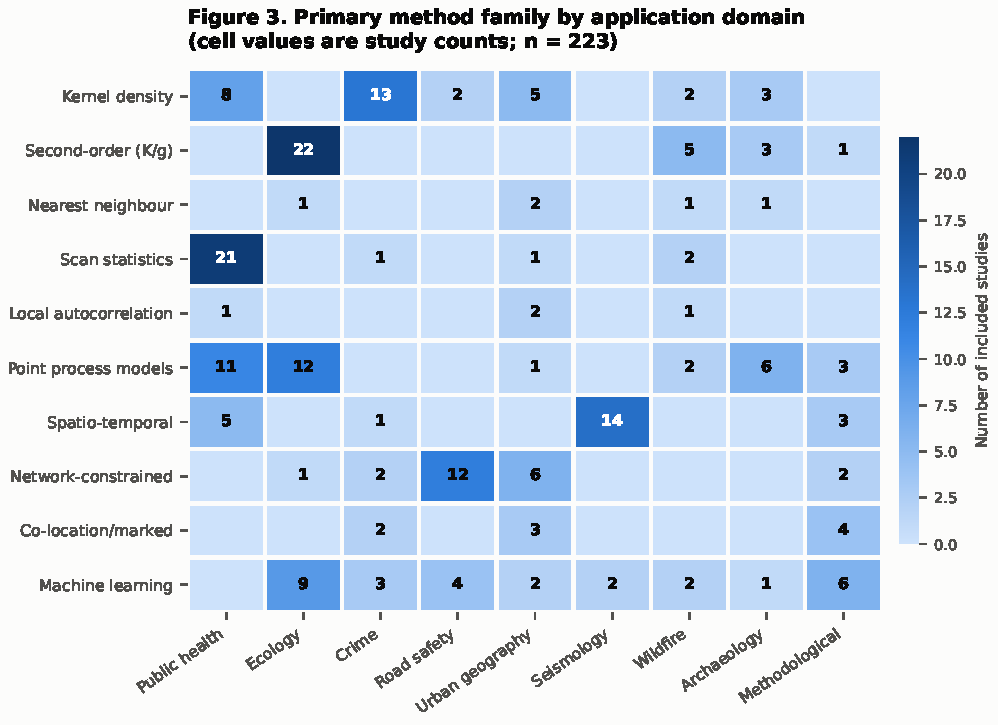
\includegraphics[width=\linewidth]{fig03_method_domain_heatmap.pdf}
\caption{Primary method family by application domain; cell values are study
counts ($n=223$).}
\label{fig:heat}
\end{figure}

Yet the off-diagonal cells are substantial, and they are where the
methodological action is. Network-constrained estimation originated in
transport and crime analysis \citep{okabe2009,yamada2007} but now appears in
roadside plant ecology \citep{spooner2004} and in retail agglomeration
analysis \citep{morioka2021,morioka2022}. Self-exciting processes moved from
seismology \citep{ogata2006,schoenberg2003} into crime forecasting
\citep{zhu2021} and epidemic modelling \citep{reinhart2017}. Presence-only
species distribution modelling was reformulated as inhomogeneous Poisson point
process estimation \citep{renner2015,phillips2009,elith2011,merow2016},
importing an entire inferential apparatus from spatial statistics into
ecology. Co-location statistics developed in economic geography
\citep{leslie2011} have been applied to crime--facility association
\citep{wang2017} and, via bivariate $K$ functions, to co-localisation in
super-resolution microscopy \citep{liu2024b}. In the opposite direction,
network-constrained co-location methods have been carried back into urban
analytics \citep{liu2021}.

The co-occurrence structure (Figure~\ref{fig:net}) shows a densely connected
core. The strongest pairings are between point process models and
spatio-temporal formulations, between kernel density estimation and
second-order statistics, and between machine learning and spatio-temporal
processes. Nearest-neighbour indices and local autocorrelation statistics sit
peripherally: they are frequently used, but as adjuncts, typically to
corroborate a density surface rather than as primary inference.

\begin{figure}[htbp]
\centering
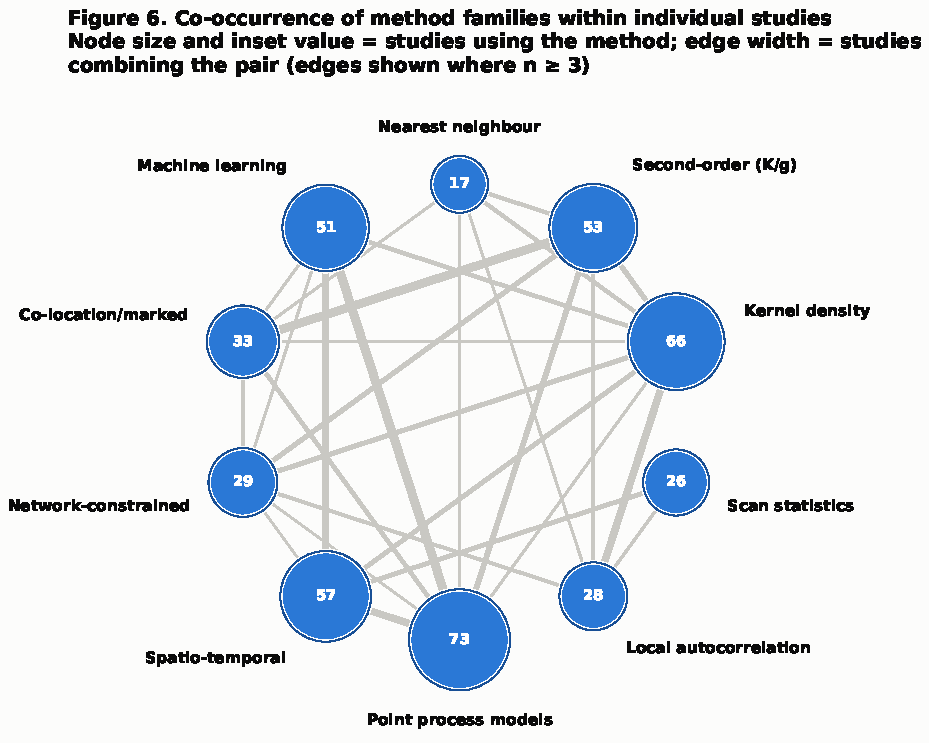
\includegraphics[width=0.9\linewidth]{fig06_method_network.pdf}
\caption{Co-occurrence of method families within individual studies. Node size
and inset value give the number of studies applying the family; edge width
gives the number of studies combining the pair (edges shown where $n\geq3$).}
\label{fig:net}
\end{figure}

\subsection{Q3 --- Methodological maturation}
Three indicators were tracked across four periods
(Figure~\ref{fig:maturity}). Methodological breadth rose sharply and then
plateaued: 57\% of pre-2006 studies combined two or more families, rising to
83\% in 2006--2012 and settling at 74--75\% thereafter. Uptake of statistical
learning is the clearest secular trend: absent before 2006, present in 17\% of
2006--2012 studies, 21\% in 2013--2019 and 26\% from 2020.

The spatio-temporal indicator behaves differently, and instructively. It was
high in the small pre-2006 group (43\%, $n=7$ --- dominated by seismological
and surveillance contributions where time is intrinsic), fell to 24\% in
2006--2012 as the field expanded through purely spatial hotspot mapping, and
has since recovered to 43\%. The dip is an expansion artefact rather than a
regression: rapid growth in cross-sectional applied mapping temporarily
diluted a temporally explicit core that has since re-established itself.

\begin{figure}[htbp]
\centering
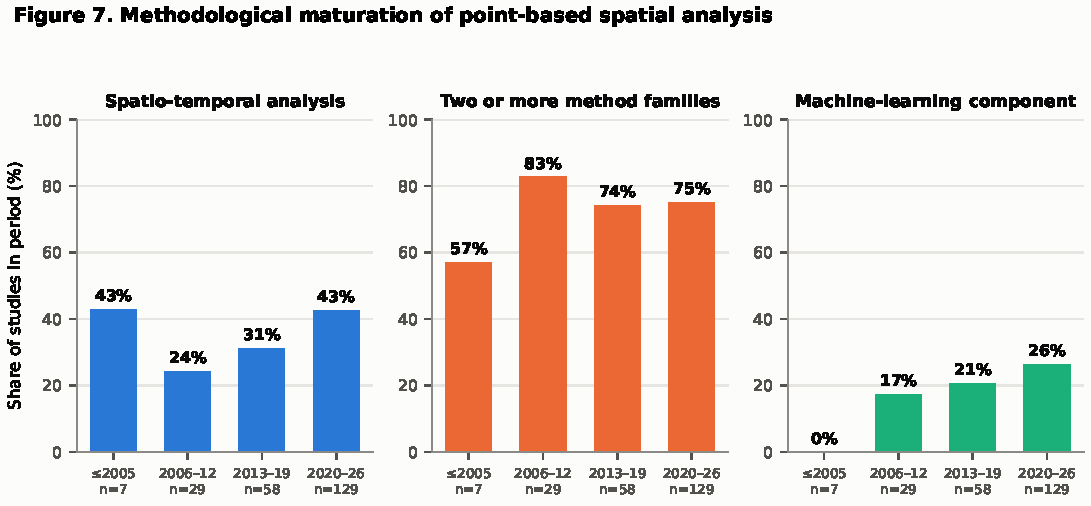
\includegraphics[width=\linewidth]{fig07_maturity.pdf}
\caption{Methodological maturation across four publication periods.}
\label{fig:maturity}
\end{figure}

Domain-level trajectories (Figure~\ref{fig:domains}) show that growth is not
uniform. Public health accelerates sharply from 2015 and again around 2020,
the latter clearly attributable to COVID-19 surveillance
\citep{desjardins2020}. Ecology grows earlier and has plateaued since about
2020. Urban geography and seismology are the steepest recent risers, the
former driven by point-of-interest datasets and the latter by neural point
process forecasting \citep{stockman2023,zlydenko2023}.

\begin{figure}[htbp]
\centering
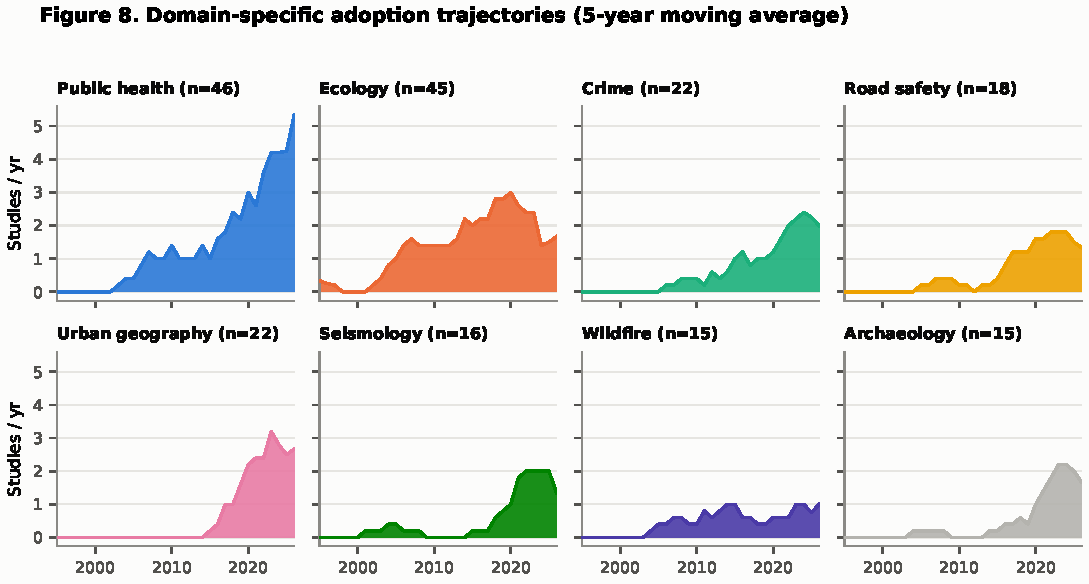
\includegraphics[width=\linewidth]{fig08_domain_trajectories.pdf}
\caption{Domain-specific adoption trajectories, five-year moving average.}
\label{fig:domains}
\end{figure}

\subsection{Q4 --- The geography of the evidence base}
Of 223 included studies, 163 could be attributed to a single case-study
country, covering 49 countries (Figure~\ref{fig:map};
Table~\ref{tab:countries}). The distribution is highly concentrated. The
United States (32 studies), China (26), the United Kingdom (13), Japan (10)
and Brazil (7) together account for 88 studies --- 54\% of all
country-attributable work. Thirty countries are represented by a single study.

\begin{figure}[htbp]
\centering
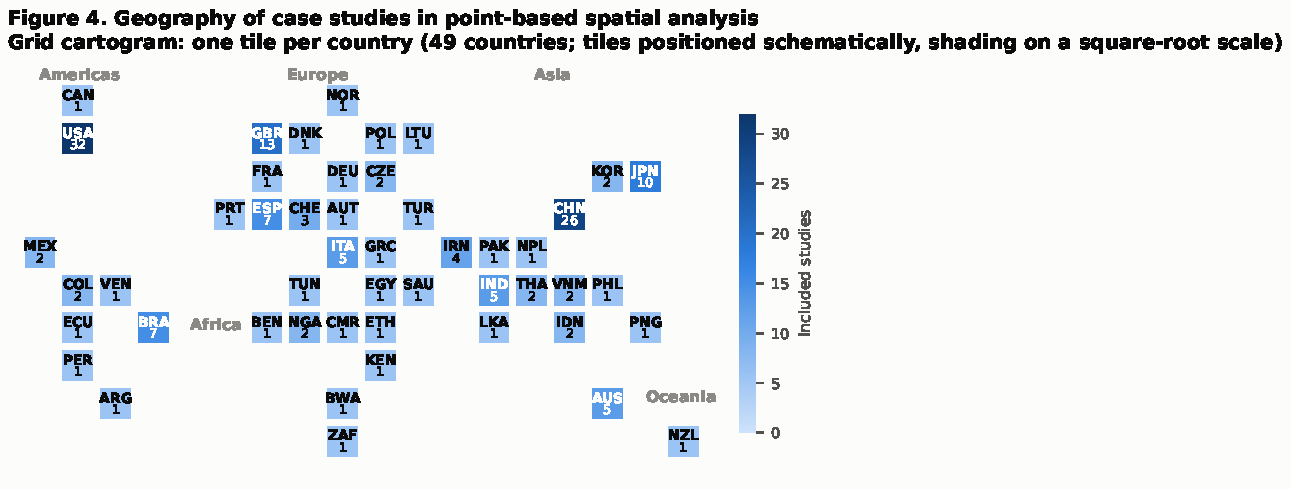
\includegraphics[width=\linewidth]{fig04_country_cartogram.pdf}
\caption{Geography of case studies. Grid cartogram with one tile per country;
tiles are positioned schematically rather than by projected coordinates so
that every country remains legible. Shading is on a square-root scale.}
\label{fig:map}
\end{figure}

Regionally, Europe (39), Eastern Asia (38) and Northern America (33) dominate;
Sub-Saharan Africa contributes 8 studies and Northern Africa 2, so the African
continent supplies 6.1\% of country-attributable work
(Figure~\ref{fig:equity}a). By income group, 56\% of attributable studies are
set in high-income countries and 1.2\% ($n=2$) in low-income countries.

\begin{figure}[htbp]
\centering
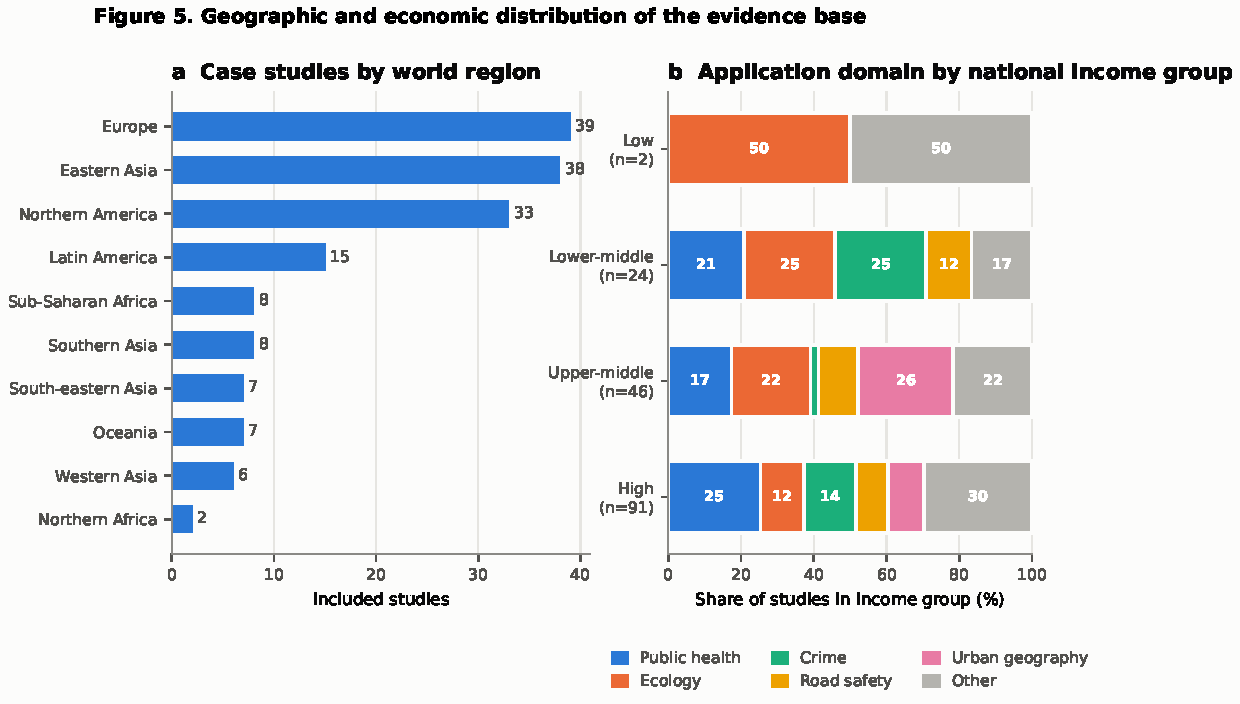
\includegraphics[width=\linewidth]{fig05_equity.pdf}
\caption{Geographic and economic distribution of the evidence base.
(a) Case studies by world region. (b) Application domain composition by
national income group.}
\label{fig:equity}
\end{figure}

The composition of research also shifts with income (Figure~\ref{fig:equity}b).
In high-income settings the portfolio is broad, with ecology, public health,
crime and urban applications all substantially represented. In lower-middle
and low-income settings the portfolio narrows towards public health and, to a
lesser extent, road safety --- a pattern consistent with donor-funded disease
surveillance driving the available georeferenced data
\citep{coleman2009,gachohi2022,tewara2018,cuadros2018}. Point-based methods
are being applied in these settings, and often creatively under severe data
constraints \citep{babaganakyari2025,mfundisi2019,mejri2026,afolayan2022},
but across a markedly narrower range of questions.

%----------------------------------------------------------------- DISCUSSION
\section{Discussion}

\subsection{Four trajectories, one shift}
Read together, the results describe four trajectories that are facets of a
single movement: point-based spatial analysis is becoming a
\emph{model-based, domain-constrained, computationally learned} enterprise.

\textbf{From description to inference.} The displacement of kernel density
estimation by point process models as the modal framework is the field's
central methodological event. It changes the object of study from a smoothed
surface to a parameterised intensity with quantified uncertainty, and it makes
covariate effects, residual diagnostics and model comparison available
\citep{diggle2013b,renner2015,merow2016}.

\textbf{From planar to constrained domains.} Thirteen per cent of studies
already work on linear networks, and the methodological literature is
unambiguous that applying planar statistics to network-constrained events is
not a minor approximation but a source of qualitatively wrong conclusions
\citep{okabe2009,baddeley2020,rakshit2017}. The choice of distance metric on
the network is itself consequential \citep{rakshit2017}.

\textbf{From statistics to learning.} Neural point processes now provide
flexible conditional intensities that outperform parametric baselines in
forecasting settings \citep{chen2020,zhou2021,stockman2023,zlydenko2023}.
The most interesting contributions are hybrids that retain an interpretable
kernel while learning its shape \citep{cheng2025,muir2023,mateu2022}, rather
than replacements of the statistical framework outright.

\textbf{From single methods to combined workflows.} Three-quarters of studies
combine families, and the standard modern workflow --- estimate intensity,
test against an inhomogeneous null, fit a parametric or learned model,
validate on held-out data --- is now visible across domains that do not cite
each other.

\subsection{What the trajectories leave unresolved}
Three problems recur across the corpus and are not being resolved by the
methodological shift.

\emph{Bandwidth and scale remain under-reported and consequential.} The
sensitivity of kernel estimates to bandwidth has been demonstrated repeatedly
\citep{chainey2014,hart2014,amatulli2007}, and shown to change substantive
conclusions: data-driven bandwidths spanning 46--48{,}450 ft produced
intervention effects that were detectable only within a narrow band, with
larger bandwidths reversing the apparent sign of an effect
\citep{zewdie2025}. Bandwidth selection is a substantive modelling decision
and should be reported and justified as one.

\emph{Positional uncertainty is systematically ignored.} Geocoding error,
address aggregation and confidentiality-driven displacement all perturb the
input to every method reviewed here. Where this has been studied, effects are
material: preprocessing strategy interacts with spatial support and degrades
hotspot prediction markedly once a substantial fraction of records is
displaced \citep{wang2026}, and network-constrained models that ignore
location uncertainty misattribute accident intensity to intersections
\citep{brizredon2023}. Very few applied studies propagate this uncertainty.

\emph{Null models are frequently mis-specified.} Testing against complete
spatial randomness in an environment that is manifestly inhomogeneous
guarantees rejection and tells the analyst nothing
\citep{law2009,wiegand2007,velazquez2016}. The same logic drives the
sampling-bias literature in presence-only modelling, where the background
sample defines the null and materially determines conclusions
\citep{phillips2009,fourcade2014,yackulic2013,elgabbas2018}. Scan statistics
carry an analogous hazard: the most likely cluster is systematically inflated
by absorbing neighbouring low-risk regions unless the likelihood is restricted
\citep{tango2021,tango2012}, and reported cluster size depends on
user-selected reporting rules \citep{han2016a}.

\subsection{The geography gap}
The concentration of case studies is severe enough to qualify the field's
empirical claims. Fifty-four per cent of country-attributable work comes from
five countries, and two studies in this corpus are set in low-income
countries. Because point-based analysis requires georeferenced individual
event data, the distribution of studies largely tracks the distribution of
address-level administrative data infrastructure, not the distribution of the
processes being studied. Wildfire, road-traffic injury and vector-borne
disease --- three of the domains best served by these methods --- have burdens
concentrated precisely where the evidence is thinnest.

The consequence is not only inequitable but technical. Methods are being
tuned, and defaults established, on dense, well-geocoded, high-income
datasets. Whether bandwidth heuristics, edge corrections and background
sampling schemes transfer to sparse, coarsely geocoded, participatory or
satellite-derived point data is largely untested. The studies here that work
under exactly those constraints --- household-survey CKDu mapping in Nigeria
\citep{babaganakyari2025}, anthrax hotspot delineation in Kenya
\citep{gachohi2022}, clinic-based HIV prevalence mapping in South Africa and
Tanzania \citep{cuadros2018}, satellite-derived fire clustering in Tunisia
\citep{mejri2026} --- are the ones best placed to answer that question, and
are correspondingly valuable.

\subsection{Reproducibility and software}
A distinct strand of the corpus consists of software and reproducibility
contributions: \texttt{spatstat} and the R ecosystem
\citep{baddeley2015,baddeley2026,gonzalez2023}, scan statistic implementations
\citep{otani2021}, and Bayesian point process packages
\citep{watson2024,palmiperales2025,naylor2023}. Their prominence is
consistent with the observation that methodological diffusion in this field
tracks software availability more closely than it tracks publication: kernel
density estimation and circular scan statistics spread rapidly because they
shipped in accessible tools, whereas network-constrained and inhomogeneous
methods diffused more slowly despite being better specified for common data.
Investment in usable implementations is therefore a methodological
intervention, not a service activity.

\subsection{Limitations}
\label{sec:limits}
Four limitations bear on interpretation.

First, and most importantly, \textbf{retrieval was not exhaustive}. Searches
were run against a federated index rather than native Scopus or Web of Science
exports, queries were natural-language rather than Boolean, and no citation
chaining or hand-searching was performed. The corpus should therefore be read
as a large, systematically assembled and fully documented \emph{sample} of the
literature, not as its complete enumeration. Because retrieval is
relevance-ranked, highly cited and recent work is likely over-represented
relative to older or lower-profile studies; the sharp post-2015 growth
reported here is real but its magnitude is probably overstated.

Second, \textbf{screening and coding were performed by a single reviewer}
without duplicate independent assessment, so inter-rater reliability could not
be estimated. The point-based/areal boundary in particular required judgement.
All decisions and reasons are published per record (Supplementary Table~S2) so
that they can be audited and revised.

Third, \textbf{coding relied on titles and abstracts} rather than full texts.
Abstracts under-report methodological detail, so secondary methods, software
and parameter choices are certainly undercounted; the ``all families'' counts
are lower bounds. Fields not reliably present in abstracts --- software,
bandwidth, edge correction, sample size --- were not extracted, which is why
no quantitative methodological-quality appraisal is reported.

Fourth, \textbf{the review was not prospectively registered}, and
bibliographic records lack volume, issue, page and DOI fields, which the
retrieval index does not expose.

\subsection{A research agenda}
Five priorities follow directly from the findings.
\begin{enumerate}\itemsep2pt
  \item \textbf{Report the decisions that determine the answer.} Bandwidth and
        its selection rule, edge correction, the null model, and the
        background or population-at-risk specification should be reported as
        standard, as effect-size and confidence-interval reporting is
        elsewhere.
  \item \textbf{Propagate positional uncertainty.} Geocoding error and
        privacy-driven displacement should be modelled, not assumed away
        \citep{wang2026,brizredon2023}.
  \item \textbf{Default to the constrained domain where events are
        constrained.} For crashes, street crime and roadside ecology, network
        formulations should be the default and planar analysis the choice
        requiring justification \citep{baddeley2020,rakshit2017}.
  \item \textbf{Build interpretable hybrids.} The productive frontier couples
        neural flexibility with retained, inspectable kernel structure
        \citep{cheng2025,mateu2022}, and should be evaluated on calibration
        and transferability, not only on predictive scores.
  \item \textbf{Invest deliberately in under-represented geographies.} This
        means data infrastructure and method validation under sparse and
        noisy geocoding, not only additional case studies.
\end{enumerate}

%---------------------------------------------------------------- CONCLUSIONS
\section{Conclusions}
Across 223 studies and five decades, point-based spatial analysis has moved
from a descriptive toolkit applied to mapped plots into a model-based
inferential framework applied to administrative, sensor and survey data at
scale. Four trajectories --- description to inference, planar to constrained,
statistics to learning, single method to combined workflow --- are visible
simultaneously in domains that largely do not cite one another, which is
strong evidence of genuine convergence on a shared methodological core rather
than parallel invention.

That convergence is incomplete in two specific ways. Methodologically, the
decisions that most affect conclusions --- bandwidth, edge correction, null
model, positional uncertainty --- remain the least consistently reported.
Empirically, the evidence base is drawn overwhelmingly from a handful of
high-income, data-rich countries, so the field's defaults have been calibrated
on conditions that do not hold where many of the relevant processes are most
consequential. Closing those two gaps, rather than adding further estimators,
is where the next decade of value lies.

%------------------------------------------------------------------ BACKMATTER
\section*{Data and code availability}
The complete extraction dataset (223 included studies with all coded fields),
the full decision log including excluded records with reasons, the PRISMA
counts, and all analysis and figure-generation code are distributed with this
manuscript in the accompanying repository.

\section*{Declaration of competing interest}
The author declares no competing interests.

\section*{Funding}
This research received no specific grant from any funding agency.

\section*{Declaration of generative AI use}
Bibliographic retrieval, record coding, quantitative synthesis and figure
generation were carried out with computational assistance. All eligibility
decisions and their reasons are published per record for independent audit.

%------------------------------------------------------------------- TABLES
\clearpage
\begin{table}[htbp]
\centering
\footnotesize
\caption{Search strategy: query identifiers, natural-language query strings issued to the federated bibliographic index, and record yield at each stage.}
\label{tab:search}
\begin{tabular}{llrrr}
\toprule
ID & Query string & Retrieved & Included & Yield (\%) \\
\midrule
S01 & point pattern analysis spatial point process methods review & 20 & 14 & 70 \\
S02 & kernel density estimation hotspot mapping crime incidents & 20 & 20 & 100 \\
S03 & spatial scan statistic disease cluster detection SaTScan & 20 & 20 & 100 \\
S04 & Ripley's K function spatial pattern forest tree species distribution & 20 & 20 & 100 \\
S05 & spatio-temporal point process earthquake ETAS self-exciting model & 20 & 19 & 95 \\
S06 & network constrained point pattern analysis road traffic accidents street network & 20 & 15 & 75 \\
S07 & log-Gaussian Cox process spatial epidemiology disease risk mapping & 20 & 17 & 85 \\
S08 & point of interest POI spatial clustering urban vitality retail location & 20 & 12 & 60 \\
S09 & wildfire ignition point pattern analysis spatial clustering & 20 & 15 & 75 \\
S10 & archaeological site distribution spatial point pattern analysis settlement & 20 & 15 & 75 \\
S11 & co-location quotient bivariate marked point pattern cross-K function & 19 & 14 & 74 \\
S12 & deep learning neural spatio-temporal point process event prediction & 19 & 11 & 58 \\
S13 & presence-only species distribution model point process MaxEnt sampling bias & 20 & 19 & 95 \\
S14 & kernel density hotspot analysis health facility disease mapping Africa sub-Saharan GIS & 20 & 12 & 60 \\
Total &  & 278 & 223 & 80 \\
\bottomrule
\end{tabular}
\begin{minipage}{\linewidth}\vspace{4pt}\scriptsize Searches were executed on 28 July 2026 against a federated index spanning Semantic Scholar, PubMed, Scopus and arXiv. Yield is the proportion of records retrieved by a query that met all eligibility criteria; records retrieved by more than one query are attributed to the first query that returned them.\end{minipage}
\end{table}

\begin{table}[htbp]
\centering
\footnotesize
\caption{Eligibility criteria applied at record screening.}
\label{tab:elig}
\begin{tabular}{p{0.13\linewidth}p{0.40\linewidth}p{0.40\linewidth}}
\toprule
Dimension & Inclusion criterion & Exclusion criterion \\
\midrule
Population & Studies analysing georeferenced event locations (points) in any application field & Studies analysing only areal/lattice aggregates, raster surfaces or extended (line, polygon) objects \\
Concept & Application or development of at least one point-based spatial statistic or point process model & Purely temporal point processes; accessibility, travel-time or suitability models with no point pattern statistic \\
Context & Any geography, spatial scale and time period & None \\
Publication type & Peer-reviewed journal article, conference paper, or preprint with a full abstract & Books, monographs, theses, book reviews, correction notices and conference abstracts without full text \\
Language & English-language abstract available & None \\
Reporting & Sufficient information in the record to code method family, application domain and study area & Records with no indexed abstract or with corrupted metadata \\
\bottomrule
\end{tabular}
\end{table}

\begin{table}[htbp]
\centering
\footnotesize
\caption{Taxonomy of point-based method families, with usage, recency and citation profile across the 223 included studies.}
\label{tab:methods}
\begin{tabular}{p{0.17\linewidth}p{0.30\linewidth}rrrrrr}
\toprule
Method family & Scope & Primary $n$ & Any use $n$ & \% of studies & Median year & Median cites & \% ST \\
\midrule
Parametric point process models & Inhomogeneous Poisson, Cox and log-Gaussian Cox, cluster and Gibbs processes; presence-only intensity models & 36 & 73 & 32.7 & 2020 & 24 & 27 \\
Kernel density estimation & Smooths event locations into a continuous intensity surface; planar, adaptive and space--time variants & 33 & 66 & 29.6 & 2022 & 15 & 41 \\
Spatio-temporal point processes & Separable and non-separable space--time intensity models; self-exciting Hawkes and ETAS formulations & 23 & 57 & 25.6 & 2022 & 14 & 98 \\
Second-order distance statistics & Ripley's $K$, $L$, pair correlation $g$, and the empty-space $F$, nearest-neighbour $G$ and $J$ functions & 31 & 53 & 23.8 & 2018 & 18 & 17 \\
Machine-learning point models & Neural point processes, density-based clustering, maximum-entropy and ensemble intensity learners & 30 & 51 & 22.9 & 2022 & 26 & 41 \\
Co-location and marked patterns & Cross-$K$, co-location quotient, mark correlation and multitype/bivariate summary functions & 10 & 33 & 14.8 & 2019 & 18 & 15 \\
Network-constrained analysis & Density and second-order statistics computed with shortest-path or other network metrics on linear networks & 23 & 29 & 13.0 & 2021 & 25 & 31 \\
Local association on points & Getis--Ord $G_i^*$ and local Moran's $I$ applied to event locations or point-derived densities & 4 & 28 & 12.6 & 2021 & 20 & 25 \\
Scan statistics & Kulldorff circular, elliptic and flexibly shaped spatial and space--time scan statistics & 25 & 26 & 11.7 & 2020 & 40 & 46 \\
Nearest-neighbour indices & Average nearest-neighbour ratio, Clark--Evans index and dispersion indices & 6 & 17 & 7.6 & 2021 & 11 & 24 \\
Other approaches & Spectral, tessellation-based, fractal and graph-analytic descriptions of point configurations & 2 & 10 & 4.5 & 2021 & 8 & 20 \\
\bottomrule
\end{tabular}
\begin{minipage}{\linewidth}\vspace{4pt}\scriptsize ``Primary'' counts studies whose dominant analytical approach falls in the family; ``any use'' counts every study applying the family, so column totals exceed 223. \% ST is the share of studies in that family with an explicit temporal dimension.\end{minipage}
\end{table}

\begin{table}[htbp]
\centering
\scriptsize
\caption{Cross-tabulation of primary method family by application domain (study counts).}
\label{tab:crosstab}
\begin{tabular}{p{0.19\linewidth}rrrrrrrrrrrrr}
\toprule
Method family & Health & Ecol. & Crime & Urban & Meth. & Road & Seism. & Fire & Arch. & Micro. & Env. & Other & Total \\
\midrule
Kernel density estimation & 8 & 0 & 13 & 5 & 0 & 2 & 0 & 2 & 3 & 0 & 0 & 0 & 33 \\
Second-order distance statistics & 0 & 22 & 0 & 0 & 1 & 0 & 0 & 5 & 3 & 0 & 0 & 0 & 31 \\
Nearest-neighbour indices & 0 & 1 & 0 & 2 & 0 & 0 & 0 & 1 & 1 & 1 & 0 & 0 & 6 \\
Scan statistics & 21 & 0 & 1 & 1 & 0 & 0 & 0 & 2 & 0 & 0 & 0 & 0 & 25 \\
Local association on points & 1 & 0 & 0 & 2 & 0 & 0 & 0 & 1 & 0 & 0 & 0 & 0 & 4 \\
Parametric point process models & 11 & 12 & 0 & 1 & 3 & 0 & 0 & 2 & 6 & 0 & 1 & 0 & 36 \\
Spatio-temporal point processes & 5 & 0 & 1 & 0 & 3 & 0 & 14 & 0 & 0 & 0 & 0 & 0 & 23 \\
Network-constrained analysis & 0 & 1 & 2 & 6 & 2 & 12 & 0 & 0 & 0 & 0 & 0 & 0 & 23 \\
Co-location and marked patterns & 0 & 0 & 2 & 3 & 4 & 0 & 0 & 0 & 0 & 1 & 0 & 0 & 10 \\
Machine-learning point models & 0 & 9 & 3 & 2 & 6 & 4 & 2 & 2 & 1 & 0 & 0 & 1 & 30 \\
Other approaches & 0 & 0 & 0 & 0 & 1 & 0 & 0 & 0 & 1 & 0 & 0 & 0 & 2 \\
Total & 46 & 45 & 22 & 22 & 20 & 18 & 16 & 15 & 15 & 2 & 1 & 1 & 223 \\
\bottomrule
\end{tabular}
\end{table}

\begin{table}[htbp]
\centering
\footnotesize
\caption{Twenty most frequently studied countries, with world region, income group and leading application domain.}
\label{tab:countries}
\begin{tabular}{lrp{0.15\linewidth}p{0.11\linewidth}rp{0.21\linewidth}}
\toprule
Country & Studies & Region & Income group & Median year & Leading domain \\
\midrule
United States & 32 & Northern America & High & 2018 & Public health and epidemiology \\
China & 26 & Eastern Asia & Upper-middle & 2022 & Urban and economic geography \\
United Kingdom & 13 & Europe & High & 2022 & Public health and epidemiology \\
Japan & 10 & Eastern Asia & High & 2020 & Urban and economic geography \\
Brazil & 7 & Latin America & Upper-middle & 2019 & Ecology, forestry and biodiversity \\
Spain & 7 & Europe & High & 2019 & Road safety and transport \\
Australia & 5 & Oceania & High & 2011 & Ecology, forestry and biodiversity \\
India & 5 & Southern Asia & Lower-middle & 2023 & Crime and policing \\
Italy & 5 & Europe & High & 2020 & Seismology \\
Iran & 4 & Western Asia & Lower-middle & 2021 & Ecology, forestry and biodiversity \\
Switzerland & 3 & Europe & High & 2018 & Public health and epidemiology \\
Czech Republic & 2 & Europe & High & 2013 & Public health and epidemiology \\
Colombia & 2 & Latin America & Upper-middle & 2024 & Road safety and transport \\
Thailand & 2 & South-eastern Asia & Upper-middle & 2025 & Public health and epidemiology \\
South Korea & 2 & Eastern Asia & High & 2018 & Public health and epidemiology \\
Vietnam & 2 & South-eastern Asia & Lower-middle & 2019 & Road safety and transport \\
Indonesia & 2 & South-eastern Asia & Lower-middle & 2020 & Seismology \\
Nigeria & 2 & Sub-Saharan Africa & Lower-middle & 2023 & Public health and epidemiology \\
Mexico & 2 & Latin America & Upper-middle & 2022 & Ecology, forestry and biodiversity \\
Ethiopia & 1 & Sub-Saharan Africa & Low & 2022 & Archaeology and heritage \\
\bottomrule
\end{tabular}
\begin{minipage}{\linewidth}\vspace{4pt}\scriptsize 49 distinct countries appear across 163 of the 223 included studies; the remainder are methodological contributions, simulation studies or multi-country analyses with no single case-study country.\end{minipage}
\end{table}

\begin{table}[htbp]
\centering
\footnotesize
\caption{Characteristics of the 223 included studies.}
\label{tab:characteristics}
\begin{tabular}{p{0.55\linewidth}r}
\toprule
Characteristic & $n$ (\%) \\
\midrule
Total included studies & 223 (100.0) \\
\textit{Publication period} &  \\
\quad 1977--2005 & 7 (3.1) \\
\quad 2006--2012 & 29 (13.0) \\
\quad 2013--2019 & 58 (26.0) \\
\quad 2020--2026 & 129 (57.8) \\
\textit{Document type} &  \\
\quad Article & 190 (85.2) \\
\quad Review & 16 (7.2) \\
\quad Conference & 8 (3.6) \\
\quad Preprint & 9 (4.0) \\
\textit{Temporal dimension} &  \\
\quad Purely spatial & 140 (62.8) \\
\quad Spatio-temporal & 83 (37.2) \\
\textit{Methodological breadth} &  \\
\quad Single method family & 55 (24.7) \\
\quad Two method families & 125 (56.1) \\
\quad Three or more & 43 (19.3) \\
\textit{Geographic attribution} &  \\
\quad Single case-study country & 163 (73.1) \\
\quad Multi-country & 23 (10.3) \\
\quad Not attributable / simulation & 37 (16.6) \\
\textit{National income group (attributable studies)} &  \\
\quad High income & 91 (55.8) \\
\quad Upper-middle income & 46 (28.2) \\
\quad Lower-middle income & 24 (14.7) \\
\quad Low income & 2 (1.2) \\
\textit{Citation impact} &  \\
\quad Median citations (IQR) & 18 (3--70) \\
\bottomrule
\end{tabular}
\begin{minipage}{\linewidth}\vspace{4pt}\scriptsize Percentages within the income-group block are computed over the subset of studies attributable to a single country.\end{minipage}
\end{table}


\clearpage
\bibliography{references}

\end{document}
